\documentclass[12pt]{article}

\usepackage[a4paper, margin=1in]{geometry}
\usepackage{graphicx}
\usepackage{float}
\usepackage{hyperref}

\hypersetup{
    colorlinks=true,   
    urlcolor=cyan
}

\setlength\parindent{0pt}
\setlength\parskip{1em}

\title{System Architectures \\ \bigskip Centralized Chat System}
\author{\textsc{Nguyen} Duc Tung \\ ICT.M7.003}
\date{\textsc{Tran} Giang Son - \textsc{Daniel} Hagimont \\ \medskip
March 26, 2018}

\begin{document}

\maketitle

\section{Introduction}

In this project, I developed a functional IRC system, with the required architecture. I tried to prevent and handle as many runtime errors could happen as I can. The system supports broadcast in a channel, send private message (PM) to a specific client. It also provides commands for client and server to utilise the system. Both server and client work with multiplexed, nonblocking TCP socket connection.

There is a short clip (1:30 mins) that demo my system: \url{https://youtu.be/vtqJ2ZCUiHs}

\section{Client}

The client firstly takes server hostname from STDIN or from arguments, and then try to connect. After successfully connected, the program creates two separated threads: input handling thread, and network handling thread. Input thread send messages from keyboard to network thread through a pipe.

The pseudo design is as follows:

\begin{figure}[H]
\centering
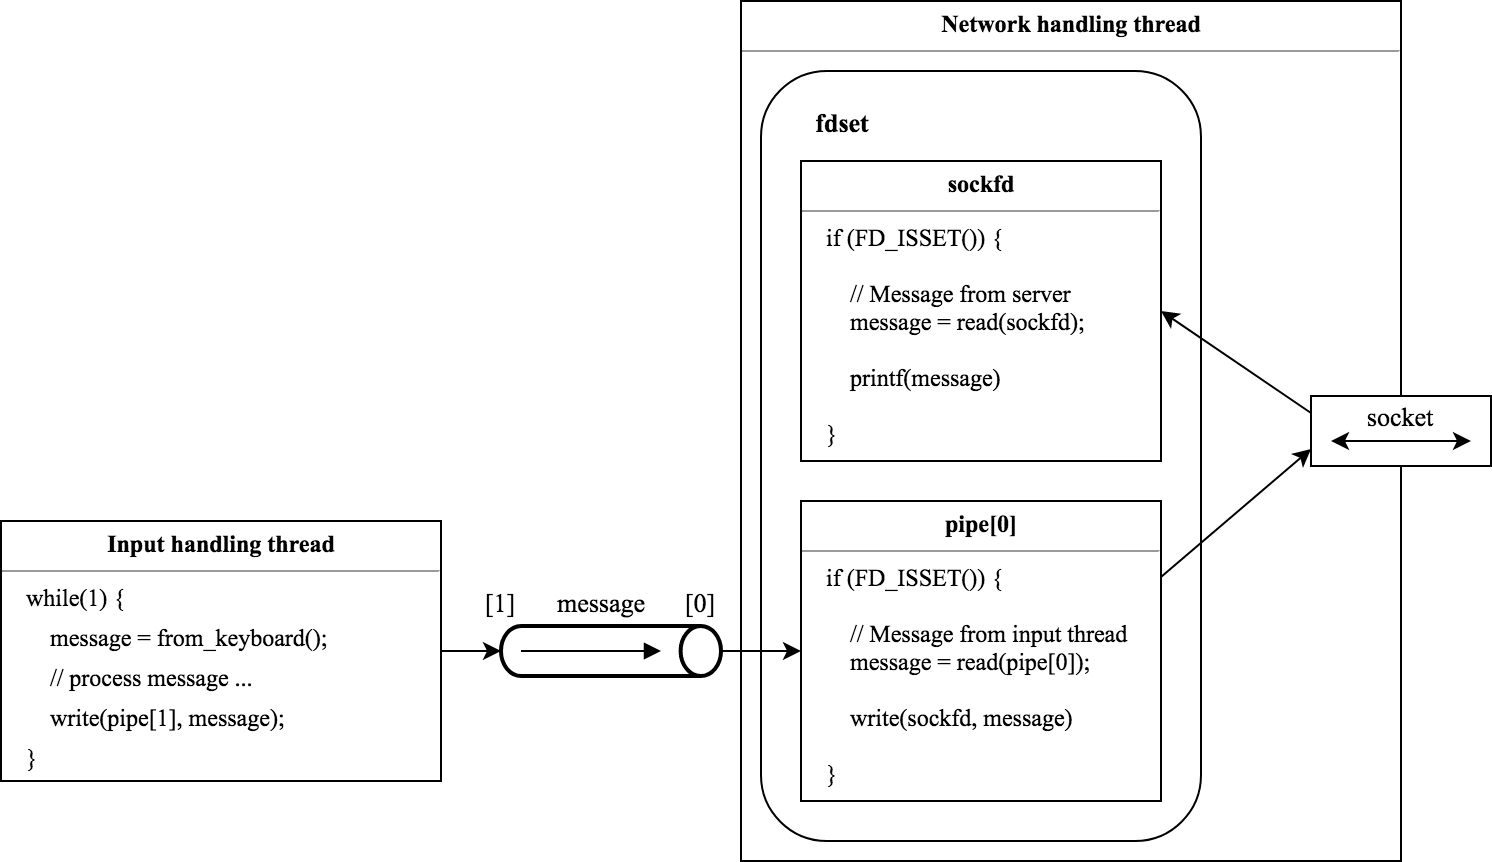
\includegraphics[width=\textwidth]{client_diagram.png}
\caption{Client's thread diagram}
\end{figure}

\subsection{Input handling thread}

The input handling thread continously getting message input from keyboard by user. The message runs through some processing such as remove `\textbackslash n' at the end, \dots After processed, message is sent to the pipe to be read by the network thread.

\subsection{Network handling thread}

The network handling thread have a \textbf{fdset} for multiplexed connection. The set include two file descriptors:

\begin{enumerate}
\item \textbf{pipe[0]}: The read-end of the pipe between input thread and this thread. It is signaled when there are messages from the input thread. If the messages are successfully received, it will be send to the server.
\item \textbf{sockfd}: The socket file descriptor, it is signaled when there are messages from the server or when the connection is closed. If there are messages, it will be printed to the terminal. Otherwise, the program will stop.
\end{enumerate}

\section{Server}

\subsection{Overall design}

The server will listen on a specific port for new connection. For each connection, it creates a child process to serve the client. A pair of pipe is used for each child process to communicate with the parent.

\begin{figure}[H]
\centering
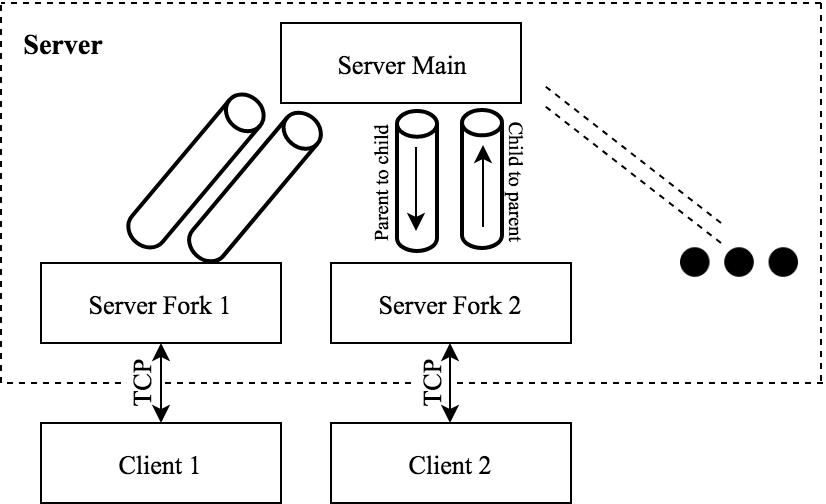
\includegraphics[width=0.75\textwidth]{server_diagram.png}
\caption{Server's design}
\end{figure}

\subsection{Main process}

\subsection{Child processes}

\subsection{Client command}

\subsection{Server command}

\end{document}